\section{Dinámica} \label{sec:dinamica}

El análisis dinámico de un robot es fundamental para entender cómo las fuerzas internas y externas afectan su movimiento. A diferencia de la cinemática, que solo considera la geometría del movimiento, la dinámica toma en cuenta las masas, fuerzas, y torques involucrados. El modelo dinámico estándar de un robot manipulador se describe mediante la ecuación:

\begin{figure}[H]
    \centering
    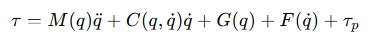
\includegraphics[width=0.75\textwidth]{img/Ecuacion Dinamica.jpeg}
    \caption{Ecuacion Dinamica}
    \label{fig:Ecuacion Dinamica}
\end{figure}

\textbf{Donde:}
\begin{itemize}
    \item T es el vector de torques articulares datos de un sensor ultrasónico o una cámara.
    \item q son el vector de posición, velocidad y aceleración articular
    \item M(q) es la matriz de masa o inercia
    \item C(q) es la matriz de Coriolis y centrífuga
    \item G(q) es el vector de gravedad
    \item F(q) representa las fuerzas de fricción
    \item Son las perturbaciones externas
\end{itemize}

\subsection{Matriz de masa o inercia}
La matriz de masa o inercia M(q) representa cómo las masas de los eslabones del robot afectan la respuesta dinámica al aplicar una aceleración. Esta matriz es simétrica, positiva definida y varía con la configuración articular del robot.

El vector de inercia determina la aceleración máxima que el sistema puede alcanzar ante una fuerza o torque dado. Si el robot se encuentra en una configuración en la que la inercia es alta por ejemplo, cuando sus eslabones están extendidos, se requerirá un mayor torque para producir una misma aceleración. Por tanto, esta matriz es clave para diseñar controladores eficientes y para limitar esfuerzos mecánicos en el sistema.

\textbf{Propiedades:}
\begin{itemize}
    \item Siempre es simétrica y positiva definida.
    \item Si el robot está en una configuración compleja (por ejemplo, extendido), la matriz tendrá valores grandes que reflejan mayor esfuerzo para moverse.
\end{itemize}

\subsection{Matriz de coriolis}

\subsection{Vector de gravedad}

Expliquen por qué el vector de gravedad en su valor máximo (cuando el robot está extendido horizontalmente) debe ser contrarrestado con la fuerza de cada motor

\subsection{Fricción}
Expliquen qué es la fricción en general.

\subsubsection{Fricción estática o seca}

\subsubsection{Fricción dinámica o viscosa}

\subsection{Perturbaciones}
Aquí expliquen qué es una perturbación en general sin profundizar mucho.